\subsection{Funciones Características Suaves y Particiones de la Unidad} \label{Subsección: Funciones Características Suaves y Particiones De La Unidad}
En esta subsección estudiaremos un conjunto de herramientas que nos serán de utilidad más adelante, las relativas a la partición de la unidad. La partición de la unidad nos permite extender funciones que estén definidas de manera local en una variedad suave de modo que estas sean suavemente cero fuera de sus dominios y de tal manera que podamos sumarlas obteniendo una función que esté definida globalmente.

\begin{definition}[Soporte De Una Función]\label{Definición: Soporte de una Función}
	Sean $M$ una variedad suave y $f: M \to \R^n$ una función suave. Definimos el \it{soporte de} $f$ como la cerradura del conjunto donde $f$ no sea anula, i.e.,

	\[ \sup f = \overline{ \{ p \in M : f(p) \neq 0 \}} \]

	Si $U \subseteq M$ y $\sup f \subseteq U$ diremos que $f$ \it{está soportada} o \it{tiene soporte en} $U$, y, si $\sup f$ es un conjunto compacto diremos que $f$ tiene \it{soporte compacto}.
\end{definition}

\begin{definition}[Función Indicadora Suave]\label{Definición: Función Indicadora Suave}
	Sea $M$ una variedad suave, $p \in M$ un punto arbitrario y $U$ una vecindad de $p$. Diremos que $f$ es una \it{función indicadora suave en $p$ con soporte en} $U$ si $f$ es una función suave con soporte en $U$ y $f$ es igual a $1$ en una vecindad de $p$.
\end{definition}


En el siguiente ejemplo construiremos una función indicadora suave.

\begin{example}\label{Ex: Función Indicadora}
	Consideremos la función por partes $f: \R \to \R$:
	\[ f(t) =
		\begin{cases}
			e^{-\frac{1}{t}} & t > 0    \\
			0                & t \leq 0
		\end{cases}
		\qquad \qquad
		\begin{gathered}
			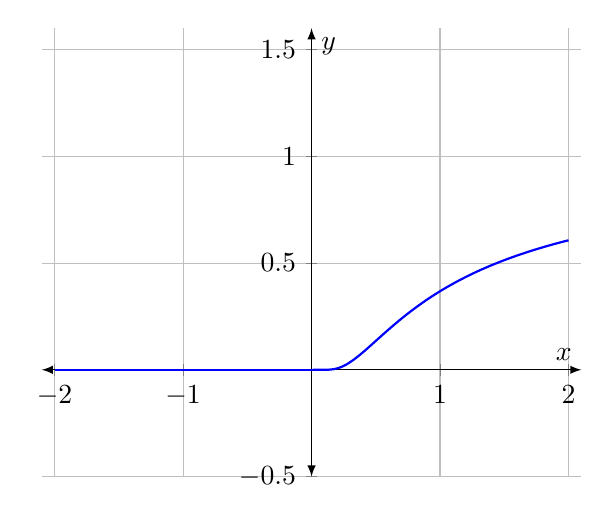
\begin{tikzpicture}
\begin{axis}[
  grid=both,
  xmin=-2.1,
  xmax=2.1,
  ymin=-0.5,
  ymax=1.6,
  axis lines=middle,
  xlabel = $x$,
  ylabel = $y$,
  axis line style={latex-latex},
  ]

\addplot[
  samples=100,
  domain=0.01:2,
  color=blue,
  thick,
  smooth,
  ]
  {(e)^(-1/x)};


\addplot[
  samples=2,
  domain=-2:0.01,
  color=blue,
  thick,
  smooth
  ]
  {0};

\end{axis}
\end{tikzpicture}

		\end{gathered}
	\]

	Comenzaremos mostrando que esta función es suave, procederemos en dos pasos:

	\begin{enumerate}
		\item La función es continua. Esto se tiene trivialmente calculando los límites laterales del cociente de Newton:
		      \begin{align*}
			      \lim_{t \to 0^+} \frac{f(t) - f(0)}{t} & = \lim_{t \to 0^+} \frac{e^{-\frac{1}{t}}}{t} = 0 \\
			      \lim_{t \to 0^-} \frac{f(t) - f(0)}{t} & = 0
		      \end{align*}
		\item Si $t > 0$, entonces la derivada $f^{(k)}$ tiene la forma $f^{(k)}(t) = p_k(t)\frac{e^{-\frac{1}{t}}}{t^{2k}}$ para algún polinomio $p_k$ con grado a lo más $k$.

		      Para $k = 0$ esto se cumplirá por definición de $f$. Supongamos que la propiedad se cumple para algún $k \geq 0$. Mostraremos que se cumple también para $f^{(k+1)}$:
		      \begin{align*}
			      f^{(k+1)}(t) & = \frac{d}{dt} f^{(k)}(t) = \frac{d}{dt} p_k(t) \frac{e^{-\frac{1}{t}}}{t^{2k}}                                                          \\
			                   & = p'_k(t) \frac{e^{-\frac{1}{t}}}{t^{2k}} + p_k(t) \frac{t^{-2} e^{-\frac{1}{t}}}{t^{2k}} - 2kp_k(t) \frac{e^{-\frac{1}{t}}}{t^{2(k+1)}} \\
			                   & = \left(t^2p'_k(t) + p_k(t) - 2ktp_k(t) \right) \frac{e^{-\frac{1}{t}}}{t^{2(k+1)}}
		      \end{align*}

		\item Claramente cuando tomamos los límites $\lim_{t \to 0^+} f^{(k)}(t)$ y $\lim_{t \to 0^-} f^{(k)}(t)$ ambos son cero.
	\end{enumerate}

	Por lo tanto $f$ es una función suave en todo $\R$

	Ahora, lo que queremos es utilizar la función $f$ para definir una función indicadora suave, el primer paso para poder lograr esto es definir la función $g: \R \to \R$ del siguiente modo:
	\[
		g(t) = \frac{f(t)}{f(t)+f(1-t)}
		\qquad \qquad
		\begin{gathered}
			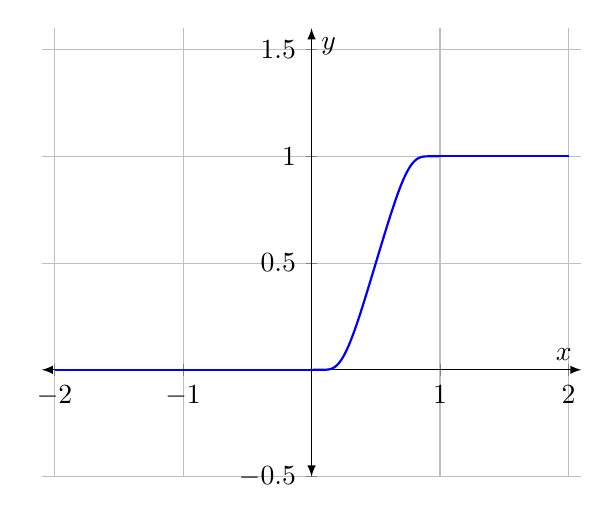
\begin{tikzpicture}
\begin{axis}[
  grid=both,
  xmin=-2.1,
  xmax=2.1,
  ymin=-0.5,
  ymax=1.6,
  axis lines=middle,
  xlabel = $x$,
  ylabel = $y$,
  axis line style={latex-latex},
  ]

\addplot[
  samples=100,
  domain=0.01:0.99,
  color=blue,
  thick,
  smooth,
  ]
  {((e)^(-1/x)) / ( ( e^(-1/x) ) + (e^(-1/(1-x))) )};


\addplot[
  samples=2,
  domain=-2:0.01,
  color=blue,
  thick,
  smooth
  ]
  {0};

\addplot[
  samples=2,
  domain=0.99:2,
  color=blue,
  thick,
  smooth
  ]
  {1};
\end{axis}
\end{tikzpicture}

		\end{gathered}
	\]


	Al ser $g$ el cociente de dos funciones suaves, y dado que el denominador no se anula en ningún punto, $g$ estará bien definida en todo $\R$, además será suave. Lo que esta función $g$ nos da es una transición suave del $0$ al $1$, por lo cual, será sencillo construir una función indicadora suave a partir de esta, esto se logrará aplicando transformaciones sencillas.

	Si tomamos $a,b \in \R$ tales que $a<b$, podemos hacer un cambio de variables del conjunto compacto $[a^2,b^2]$ al conjunto $[0,1]$ del siguiente modo:

	\[
		x \mapsto \frac{x - a^2}{b^2 - a^2}
	\]

	Esta transformación nos permite cambiar la escala de $g$  y trasladarla en el eje horizontal; es por esta razón que se define $h: \R \to \R$ del siguiente modo,
	\[
		h(x) = g\left(\frac{x - a^2}{b^2 - a^2}\right)
		\qquad \qquad
		\begin{gathered}
			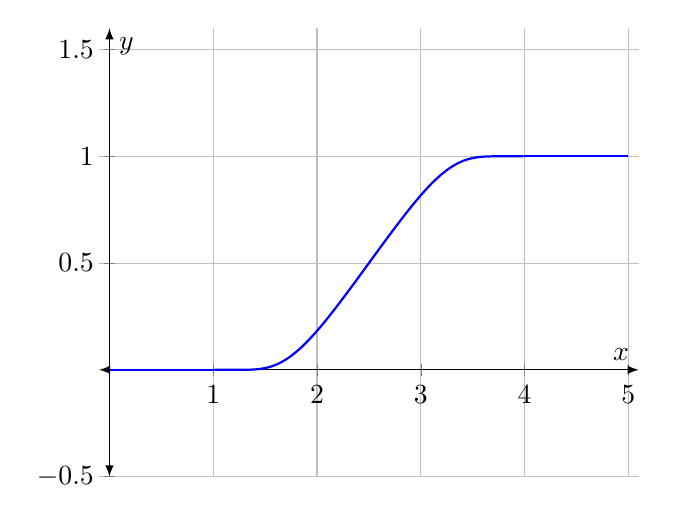
\begin{tikzpicture}
\begin{axis}[
  grid=both,
  xmin=-0.1,
  xmax=5.1,
  ymin=-0.5,
  ymax=1.6,
  axis lines=middle,
  xlabel = $x$,
  ylabel = $y$,
  axis line style={latex-latex},
  ]

\addplot[
  samples=100,
  domain=1.01:3.99,
  color=blue,
  thick,
  smooth,
  ]
  {((e)^(-1/ ((x - 1) / (4 - 1)) )) / ( ( e^(-1/ ((x - 1) / (4 - 1))) ) + (e^(-1/(1- ( (x - 1) / (4 - 1) )))) )};


\addplot[
  samples=2,
  domain=0:1.01,
  color=blue,
  thick,
  smooth
  ]
  {0};

\addplot[
  samples=2,
  domain=3.99:5,
  color=blue,
  thick,
  smooth
  ]
  {1};
\end{axis}
\end{tikzpicture}

		\end{gathered}
	\]

	Y de este modo al tomar $a,b \in \R$ cómo se acaba de hacer se tendrá que para $h$ se cumple lo siguiente

	\[
		h(x) = \begin{cases}
			1, & x > b^2    \\
			0, & x \leq a^2
		\end{cases}
	\]

	Ahora, podemos tomar $k(x)=h(x^2)$ para hacer que nuestra función sea simétrica alrededor del origen.

	\[
		k(x) = h(x^2) = g\left(\frac{x^2 - a^2}{b^2 - a^2}\right)
		\qquad \qquad
		\begin{gathered}
			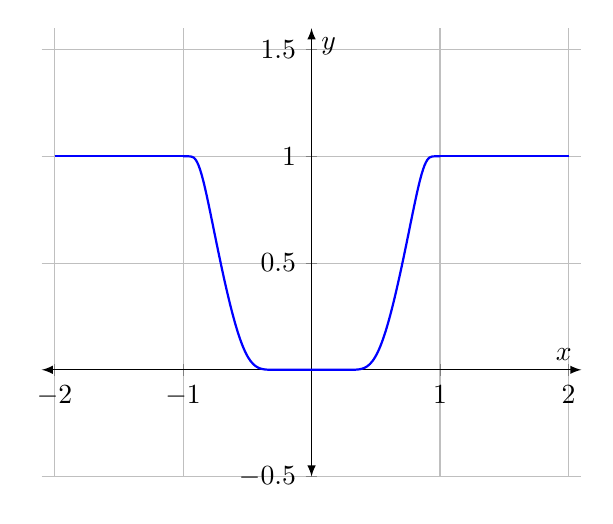
\begin{tikzpicture}
\begin{axis}[
  grid=both,
  xmin=-2.1,
  xmax=2.1,
  ymin=-0.5,
  ymax=1.6,
  axis lines=middle,
  xlabel = $x$,
  ylabel = $y$,
  axis line style={latex-latex},
  ]

\addplot[
  samples=100,
  domain=-1:1,
  color=blue,
  thick,
  smooth,
  ]
  {((e)^(-1/(x^2))) / ( ( e^(-1/(x^2)) ) + (e^(-1/(1-(x^2)))) )};


\addplot[
  samples=2,
  domain=-2:-0.99,
  color=blue,
  thick,
  smooth
  ]
  {1};

\addplot[
  samples=2,
  domain=0.99:2,
  color=blue,
  thick,
  smooth
  ]
  {1};
\end{axis}
\end{tikzpicture}

		\end{gathered}
	\]



	Y finalmente, definimos la función suave $r$ de modo que su valor sea $1$ en el intervalo y $0$ fuera de este haciendo un pequeño ajuste del siguiente modo.
	\[
		r(t) = 1 - k(x) = 1 - g\left(\frac{x^2 - a^2}{b^2 - a^2}\right)
		\qquad \qquad
		\begin{gathered}
			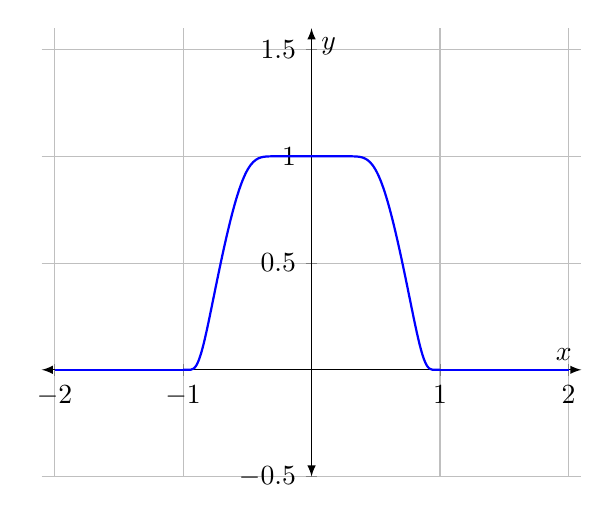
\begin{tikzpicture}
\begin{axis}[
  grid=both,
  xmin=-2.1,
  xmax=2.1,
  ymin=-0.5,
  ymax=1.6,
  axis lines=middle,
  xlabel = $x$,
  ylabel = $y$,
  axis line style={latex-latex},
  ]

\addplot[
  samples=100,
  domain=-1:1,
  color=blue,
  thick,
  smooth,
  ]
  {1 -( ((e)^(-1/(x^2))) / ( ( e^(-1/(x^2)) ) + (e^(-1/(1-(x^2)))) ))};


\addplot[
  samples=2,
  domain=-2:-0.99,
  color=blue,
  thick,
  smooth
  ]
  {0};

\addplot[
  samples=2,
  domain=0.99:2,
  color=blue,
  thick,
  smooth
  ]
  {0};
\end{axis}
\end{tikzpicture}

		\end{gathered}
	\]

	$r(t)$ es una función indicadora suave en $0$  y para cualquier $q \in \R$ tenemos que $r(x-q)$ es una función indicadora en $q$. Esta idea puede ser extendida a $\R^n$ como una función indicadora suave en $0 \in \R^n$  cuyo valor es $1$ en la bola (cerrada) $B_a(0)$ y $0$ fuera de la bola $B_b(0)$ si tomamos la función $r: \R^n \to \R$ cómo:

	\[
		\sigma(x) = r(\|x\|) = 1 - g\left(\frac{\|x\| - a^2}{b^2 - a^2}\right)
	\]
\end{example}

\begin{figure}
	\centering
	\begin{tikzpicture}[scale=1.25]
	\begin{axis}[
      view={30}{30},
			colormap/cool,
			xmin=-2,
			xmax=2.5,
			ymin=-2.5,
			ymax=2,
			zmin=-0.25,
			zmax=1.5,
			% axis lines=middle,
		]
		\addplot3[
			domain=-1.9:2.4,
			domain y = -2.4:1.9,
			patch,
			patch type=bilinear,
			shader=faceted interp,
		]
		{abs(x^2 + y^2) < 1 ? e^(-1 / (1 - abs(x^2 + y^2)) ) : 0 };

	\end{axis}
\end{tikzpicture}

	\caption{Representación de una función indicadora suave en $\R^2$}
\end{figure}


Lo que haremos a continuación será extender estas ideas, mostraremos que para un cualquier punto en una variedad y cualquier vecindad que contenga a ese punto podemos encontrar una función indicadora suave en el punto con soporte en la vecindad.

\begin{lemma}\label{Lemma: Existencia de Función Indicadora}
	Sea $M^n$ una variedad suave, $p \in M$ un punto arbitrario y $U \subseteq M$ una vecindad de $p$. Entonces existe una función indicadora suave en $p$ con soporte en $U$.
\end{lemma}

\begin{proof}
	Sea $a$ un punto arbitrario en $M$ y $U$ una vecindad de $q$. Por ser $M$ una variedad suave existirá una carta suave $(V,\psi)$ que contiene a $q$ y tal que $V \subset U$.

	Consideremos la función $\sigma: \R^n \to \R$ definida anteriormente. $\sigma$ es una función indicadora suave en $\psi(q)$ con soporte en una bola compacta $B_r(\psi(q)) \subset V$. Definimos la función

	\[
		f(p) = \begin{cases}
			\sigma(\psi(p)), & p \in V    \\
			0,               & p \notin V
		\end{cases}
	\]

	Mostraremos que, en efecto, esta función es una función indicadora en $q$ con soporte en $U$.

	Por como hemos construido a $\sigma$, esta tiene soporte compacto, esto es, $\sup \sigma$ es un conjunto compacto, luego $\psi^{-1}(\sup \sigma)$ será la imagen continua de un conjunto compacto, i.e., $\psi^{-1}(\sup \sigma)$ es un compacto en $M$. Dado que $M$ es Hausdorff podemos garantizar que $\psi^{-1} (\sup \sigma)$ es cerrado. Por lo tanto, tendremos que
	\[
		\sup f \subset \phi^{-1} (\sup \sigma) \subset V
	\]

	Es claro que si $p \in V$, $f$ es suave en $p$ dado que $f(p)$ será la imagen de la composición de dos funciones suave. En el caso contrario, si $p \notin V$, entonces podremos elegir una carta $(W,\omega)$ que contengan a $p$ y tal que $W \cap \psi^{-1}(\sup \sigma) = \varnothing$. Esta carta será también disjunta de $\sup f$, por lo que $f(W) \equiv 0$, así $f$ es una función suave, la cual es idénticamente $1$ en una vecindad de $V \subset U$ de $p$ y $\sup f \subset U$. Por lo tanto, $f$ es una función indicadora suave en $q$ con soporte en $U$.
\end{proof}

\begin{lemma}
	Sea $M$ una variedad suave, $q$ un punto arbitrario, $U \subset M$ una vecindad de $q$ y $f$ una función indicadora suave en $q$ con soporte en $U$. Existe una función suave $\hat{f}$ en $M$ que coincide con $f$ en alguna vecindad, posiblemente más pequeña, que contiene a $q$.
\end{lemma}

\begin{proof}
	Si tomamos una función indicadora suave $r: \R^n \to \R$ cómo se construyó en el ejemplo \ref{Ex: Función Indicadora} de tal modo que $r$ tenga soporte en $U$ y esté definida en una vecindad $V$ de $q$, podemos definir la función:
	\[
		\hat{f} = \begin{cases}
			r(x)f(x), & x \in U    \\
			0,        & x \notin U
		\end{cases}
	\]

	Dado que $\hat{f}$ es el producto de funciones suaves en $U$, $\hat{f}$ es suave en $U$. Si $x \notin U$, entonces $x \notin \sup r$, por lo que existirá una vecindad que contiene a $x$ en la cual $\hat{f}$ se anula dado que, como se vio en el lema anterior, podemos tomar $\sup r$ cerrada. Por lo tanto $\hat{f}$ es suave en cada punto $x \notin U$. Y, dado que $r \equiv 1$ en $V$, la función $\hat{f}$ coincide con $f$ en $V$.
\end{proof}

Ahora utilizaremos algunos de los resultados que pueden ser encontrados en el Anexo \ref{Anexo: Topologia De Variedades} para poder dar las siguientes definiciones.

\begin{definition}[Partición de la Unidad Subordinada]\label{Definición: Partición de la Unidad Subordnada}
	Sea $M$ una variedad suave, y sea $\mathcal{U} = \{ U_\alpha \}_{\alpha \in A}$ una cubierta abierta de $M$. Una \it{partición de la unidad suave y subordinada a} $\mathcal{U}$ es una familia $\{ \phi_{\alpha} \}_{\alpha \in A}$ formada por funciones suaves y no negativas $\phi_{\alpha} : M \to \R$ tales que
	\begin{enumerate}
		\item $\sup \phi_\alpha \subseteq U_\alpha$, para cada $\alpha \in A$.
		\item La colección $\{\sup \phi_\alpha \}_{\alpha \in A}$ es localmente finita.
		\item $\sum_{\alpha \in A} \phi_\alpha (p) = 1$ para cada $p \in M$.
	\end{enumerate}
\end{definition}

Notemos que en el tercer punto de nuestra definición no tendremos problemas de convergencia dado que, por la segunda condición, al pedir que la colección de soportes de las funciones sea localmente finita, cada punto tendrá una vecindad $V$ que interceptará a $\{\sup \phi_{\alpha}\}_{\alpha \in A}$ en un subconjunto finito de $A$, por lo que la suma será finita.

\begin{theorem}[Existencia de Particiones Suave de la Unidad]\label{Teorema: Existencia de Particiones Suave de la Unidad}
	Sea $M$ una variedad suave y sea $\mathcal{U} = \{U_\alpha\}_{\alpha \in A}$ una cubierta abierta de $M$. Existe una partición suave de la unidad subordinada a $\mathcal{U}$.
\end{theorem}

\begin{proof}
	Por el resultado mostrado en el ejemplo \ref{Ex: Variedad Suave - Subvariedades Suaves}, $U_\alpha$ es en sí misma una subvariedad suave de $M$, y por los lemas \ref{Lemma: Bolas Precompactas} y \ref{Lemma: Base Por Bolas Suaves}, cada $U_\alpha$ tendrá una base $\mathcal{B}_\alpha$ formada por bolas coordinadas regulares y precompactas. Evidentemente $\mathcal{B} = \cup_{\alpha \in A} \mathcal{B}_\alpha$ formará una base para la topología de $M$.

	Por el teorema \ref{Teorema: Espacios Precompactos} y el corolario \ref{Corolario: Variedades Precompactas} podemos garantizar que $\mathcal{U}$ tendrá un refinamiento $\{B_i\}$ numerable y localmente finito que consta de elementos de $\mathcal{B}$.

	No es difícil ver que si $\{B_i\}$ es una colección localmente finita, entonces la colección formada por la cerradura de estos conjuntos $\{\overline{B}_i\}$ también será localmente finita.


	Dado que cada $B_i$ es una bola regular coordinada en algún $U_\alpha$, por definición existirá una bola coordinada suave $B_i' \subseteq U_\alpha$ tal que $\overline{B}_{i} \subseteq B_i'$, y un mapa suave $\phi_i: B_i \to \R^n$ tal que $\phi_i(\overline{B}_i) = \overline{B}_{r_i}(0)$ y $\phi_i(B_i') = B_{r_i'}(0)$ para algunos $r_i, r_i' \in \R$ tales que $r_i < r_i'$. Para cada $i$ definiremos la función $f_i: M \to R$ como:

	\[
		f_i(q)= \begin{cases}
			\rho_i \circ \phi_i, & p \in B_i'    \\
			0,                   & p \notin B_i'
		\end{cases}
	\]

	Como se mostró en el lema \ref{Lemma: Existencia de Función Indicadora} estas funciones son suaves, más aún, son funciones indicadoras suaves, además $\sup f_i = \overline{B}_i$.

	Con estas funciones podemos definir la función $f: M \to \R$ como $f(p) = \sum_i f_i(x)$. Dado que los $\{B_i\}$ y $\{\overline{B}_i\}$ son localmente finitos, la suma será finita y por lo tanto convergerá. Cómo cada $f_i$ es no negativa en cada punto en $B_i$, y cada punto de $M$ está en algún $B_i$ por ser la colección una cubierta de $M$, se sigue que $f(p) > 0$ para cada $p \in M$. Y por cómo hemos definido $\rho$ cada $f_i$ estará normalizada por lo que $0 \leq f_i \leq 1$ y $\sum_i f_i \equiv 1$.

	Por último, hacemos un cambio de índices para nuestras funciones para que coincidan con los de la cubierta abierta $\mathcal{U}$. Dado que $\{B_i'\}$ es un refinamiento de $\mathcal{U}$, para cada $i$ podemos elegir algún índice $a(i) \in A$ tal que $B'_i \subseteq U_{a(i)}$. Para cada $\alpha \in A$ definimos la función $\psi_\alpha: M \to \R$ como:
	\[
		\psi_\alpha = \sum_{i : a(i) = \alpha} f_i
	\]

	Por estar cada $\psi_\alpha$ soportada en $\overline{B}_{i}$ tendremos que:
	\[
		\sup \psi_{\alpha} = \bigcup_{i: a(i)=\alpha} \subseteq U_\alpha
	\]

	Así, tendremos que la colección $\{\psi_{\alpha}\}$ es una partición de la unidad subordinada a $\mathcal{U}$.
\end{proof}

Los siguientes dos lemas nos darán maneras de extender funciones suaves utilizando particiones de la unidad, que, en nuestro caso, es nuestro principal interés.

\begin{lemma}
	Sea $M$ una variedad suave, $p \in M$, $A \subset M$ un subconjunto arbitrario que contiene a $p$ y $f: A \to \R^{k}$ una función suave. Existe una extensión suave a un conjunto abierto que contiene a $A$, esto es, existe un conjunto abierto $U \subset M$ tal que $A \subset U$ y una función $\hat{f}: U \to \R^{k}$ tal que $\hat{f}|_{A \cap U} = f$.
\end{lemma}

\begin{proof}
	Consideremos una vecindad $V_p$ y una función suave $f_p: V_p \to \R^n$ para cada $p \in A$ tal que $f_{p}|_{V_p \cap A} = f|_{V_p \cap A}$. Por el teorema anterior podemos garantizar que existe una partición suave de la unidad $\{\psi_{p}\}_{p \in A}$ subordinada a $U=\cup_{p \in A}V_p$

	Definiremos el conjunto $B = \{p \in A: p \in \sup \psi_p\}$ y la función $\hat{f}: \cup_{p \in A} V_p \to \R^n$ como:
	\[
		\hat{f}(x) = \sum_{x \in B} \psi_p(x)f_p(x)
	\]

	$\hat{f}$ será una función suave que coincide con $f$ en el conjunto $U \cap A$, y por cómo se ha definido $U$, es claro que $A \subseteq U$.
\end{proof}

Notemos sin embargo que no siempre es posible extender una función suave a un conjunto más grande, en particular esto no siempre es posible si la función está definida en un conjunto abierto dado que el comportamiento de la función puede ser arbitrario. Como un ejemplo sencillo en $\R$ podemos tomar la función trigonométrica $\tan: (-\frac{\pi}{2}, \frac{\pi}{2}) \to \R$, para esta función no existe una extensión suave a un subconjunto abierto más grande.

Es por esto que damos el siguiente lema, el cual es un resultado más fuerte que el anterior, y nos garantiza que si imponemos la condición de que $A$ es cerrado, entonces podremos extender cualquier función suave definida en $A$ a cualquier subconjunto abierto que lo contenga a $A$.


\begin{lemma}[Lema de Extensión para Funciones Suaves]\label{Lemma: Lema de Extensión para Funciones Suaves}
	Sea $M$ una variedad suave, $A \subset M$ un subconjunto cerrado y $f: A \to \R^k$ una función suave. Para cada conjunto abierto $U$ que contiene a $A$ existe una función suave $\hat{f}: M \to \R^{k}$ tal que $\hat{f}|_{A} = f$ y $\sup(\hat{f}) = U$.
\end{lemma}

\begin{proof}
	Procederemos de modo similar a la demostración anterior. Para cada $p \in A$ tomemos una vecindad $V_p$ y una función suave $\hat{f}_p: V_p \to \R^k$ tal que $\hat{f}_p|_{V_p \cap A} = f$. Dado un conjunto abierto $U$ podemos reemplazar $V_p$ por $V_p \cap U$ y suponer que $V_p \subset U$.

	La colección de conjuntos $B=\{V_p: p \in A\} \cup (M - A)$ será una cubierta abierta para $M$, por el teorema \ref{Teorema: Existencia de Particiones Suave de la Unidad} podemos garantizar que existirá una partición suave de la unidad subordinada a la cubierta. Digamos que $\{\psi_p: p \in A\} \cup \{\psi_0 \}$ es dicha partición de tal modo que $\sup \psi_p \subseteq V_p$ y $\sup \psi_0 \subseteq M - A$.

	Definimos la función $\hat{f}: M \to \R^k$ como:
	\[
		\sum_{p \in A} \psi_p(x)\hat{f}_p(x)
	\]

	Esta suma es convergente y está formada por el producto de funciones suaves por lo que será suave, además coincide con $f$ en $U \cap A$ y tiene soporte en $U$ dado que será idénticamente cero fuera de $A$.
\end{proof}
